\documentclass[]{article}
\usepackage{lmodern}
\usepackage{amssymb,amsmath}
\usepackage{ifxetex,ifluatex}
\usepackage{fixltx2e} % provides \textsubscript
\ifnum 0\ifxetex 1\fi\ifluatex 1\fi=0 % if pdftex
  \usepackage[T1]{fontenc}
  \usepackage[utf8]{inputenc}
\else % if luatex or xelatex
  \ifxetex
    \usepackage{mathspec}
    \usepackage{xltxtra,xunicode}
  \else
    \usepackage{fontspec}
  \fi
  \defaultfontfeatures{Mapping=tex-text,Scale=MatchLowercase}
  \newcommand{\euro}{€}
\fi
% use upquote if available, for straight quotes in verbatim environments
\IfFileExists{upquote.sty}{\usepackage{upquote}}{}
% use microtype if available
\IfFileExists{microtype.sty}{%
\usepackage{microtype}
\UseMicrotypeSet[protrusion]{basicmath} % disable protrusion for tt fonts
}{}
\usepackage{graphicx}
\makeatletter
\def\maxwidth{\ifdim\Gin@nat@width>\linewidth\linewidth\else\Gin@nat@width\fi}
\def\maxheight{\ifdim\Gin@nat@height>\textheight\textheight\else\Gin@nat@height\fi}
\makeatother
% Scale images if necessary, so that they will not overflow the page
% margins by default, and it is still possible to overwrite the defaults
% using explicit options in \includegraphics[width, height, ...]{}
\setkeys{Gin}{width=\maxwidth,height=\maxheight,keepaspectratio}
\ifxetex
  \usepackage[setpagesize=false, % page size defined by xetex
              unicode=false, % unicode breaks when used with xetex
              xetex]{hyperref}
\else
  \usepackage[unicode=true]{hyperref}
\fi
\hypersetup{breaklinks=true,
            bookmarks=true,
            pdfauthor={},
            pdftitle={},
            colorlinks=true,
            citecolor=blue,
            urlcolor=blue,
            linkcolor=magenta,
            pdfborder={0 0 0}}
\urlstyle{same}  % don't use monospace font for urls
\setlength{\parindent}{0pt}
\setlength{\parskip}{6pt plus 2pt minus 1pt}
\setlength{\emergencystretch}{3em}  % prevent overfull lines
\setcounter{secnumdepth}{0}

\date{}

\begin{document}

\section{abstract due date: 6 marzo}\label{abstract-due-date-6-marzo}

\section{paper due date: 13 marzo}\label{paper-due-date-13-marzo}

\section{Cartographic documents for web modeling and representation of
indoor mapping with interactive
environments}\label{cartographic-documents-for-web-modeling-and-representation-of-indoor-mapping-with-interactive-environments}

\section{Abstract}\label{abstract}

\section{Introduction}\label{introduction}

CARATTERISTICHE E SPUNTI:

\begin{itemize}
\item
  CONNESSIONE CON I SENSORI PER LA RILEVAZIONE DELLA POSIZIONE DEI
  VISITATORI
\item
\item
\end{itemize}

\ldots{}

The remainder of this document is organized as follows. In Section II is
provided an overview of the state of the art. Section III is devoted to
describe the novel cartographic document proposed, while section IV
introduces the underlying mathematical structure. Section V reports
about the tools and instruments developed specifically for the web,
focusing on software architecture, implemented algorithms and real
applications. Section VI describes one use case of both document format
and software tools. Finally Section VII proposes some conclusive remarks
and future developments.

\section{State of the art}\label{state-of-the-art}

Researches about the cartographic representation of indoor environments
are numerous and at the same time heterogeneos regarding to the
strategies applied. The information sources used are different,
depending on the approach, the produced solution can be more or less
precise. In some cases the information is obtained with automatic or
semi-automatic processes from files that describe the architectural
structure of a building such as BIM (Link a BIM) and/or IFC(Link a IFC)
(Danesi), in others image processing is used to extract topological
information from floor plan images (Panzieri). As a last approach,
descriptive parameters will be redefined from zero, as the current
representive stategies concerning a use beyond the mere consultation are
considered inappropriate. A recurring topic among the use of
carthograhic information is the indoor navigation(Panzieri, Polacch e
Danesi). The proposed approaches are very different in this case too,
and based on different strategies with some basic elements in common. A
recurrent solution is based on the representation of the routing
information as a graph having a node for each PoIs and an edge for each
connection between them. In some cases the edges are weighted in
function of euclidean distance. The detail level of the graph and hence
the effective practicalbility of the calculates paths, can vary
depending on the technique and the design choices applied, but in
general most of the proposed solutions (all those calculate paths)
retrieve information from architectual structure. An inevitably theme
connected to the navigation is the location of users. All the related
works agree on the inadequacy of GNSS in indoors contexts, due to the
segnificant redaction in the signal quality. To locate the exact
position within a building, the currently most used techniques are based
on fingerprinting and triangulation of radio signals (WiFi, Bluetooth,
etc.) flanked by more original solutions based on, for example, image
recognition (arabi). The proposed solutions for the movements tracking
range from the creation of ad hoc deviced(Panzieri) to the use of
sensors alredy present in many smartphones for inertial tracking(Arabi).

(DANESI: Boysen M. de Haas C., Lu H., Xie X., Pilvinyte A., Constructing
Indoor Navigation Systems from Digital Building Information, ICDE
Conference, pp.~1194-1197, 2014.) (ARABI: Al Delail B., Weruaga L.,
Zemerly M.J., Ng, J.W.P., Indoor localization and navigation using
smartphones augmented reality and inertial tracking, IEEE, pp.~929-932,
2013.) (POLACCHI: Gotlib D., Gnat M., Marciniak J., The Research on
Cartographical Indoor Presentation and Indoor Route Modeling for
Navigation Applications, International Conference on Indoor Positioning
and Indoor Navigation, 2012.) (PANZIERI: Faramondi L., Inderst F.,
Panzieri S., Pascucci F., Hybrid Map Building for Personal Indoor
Navigation Systems, IEEE/ASME International Conference on Advanced
Intelligent Mechatronics (AIM), pp.~646-651, 2014.) (CINESI: Bian W.,
Guo Y., Qiu Q., Research on Personalized Indoor Routing Algorithm, 13th
International Symposium on Distributed Computing and Applications to
Business, Engineering and Science, pp.~275-277, 2014 )

\subsection{GeoJSON}\label{geojson}

GeoJSON is a format for encoding a variety of geographic data
structures. GeoJSON supports the following geometry types:
\texttt{Point}, \texttt{LineString}, \texttt{Polygon},
\texttt{MultiPoint}, \texttt{MultiLineString}, and
\texttt{MultiPolygon}. Lists of geometries are represented by a
\texttt{GeometryCollection}. Geometries with additional properties are
\texttt{Feature} objects. And lists of features are represented by a
\texttt{FeatureCollection}.
\href{GeoJSON\%20spec}{http://geojson.org/geojson-spec.html}

GeoJSON is good for geographic mapping application, but not for indoor
application. There is a GeoJSON variant suitable for indoor app.

\subsection{Experiences on Indoor
JSON}\label{experiences-on-indoor-json}

\texttt{IndoorJSON} is a GeoJSON variant used by indoor.io toolset to
define indoor maps. IndoorJSON may consist of any number of Features
and/or FeatureCollections. All Features are interpreted similarly
regardless of their grouping into nested FeatureCollections. IndoorJSON
supports all GeoJSON geometry types.

\section{Advances on cartographics document
standards}\label{advances-on-cartographics-document-standards}

\textbf{HIJSON} (\textbf{H}ierarchical \textbf{I}ndoor \textbf{JSON}) is
a GeoJSON variant. A HIJSON document reveals at least three major
enhancements above the actual state of the art in indoor cartographic
documents:

\begin{enumerate}
\def\labelenumi{\arabic{enumi}.}
\itemsep1pt\parskip0pt\parsep0pt
\item
  Hierarchical structure
\item
  Metric local coordinate System
\item
  Semantic extensions
\end{enumerate}

\subsubsection{Hierarchical structure}\label{hierarchical-structure}

Unlike other formats like GeoJSON or IndoorJSON, HIJSON organizes its
elements in a hierarchical structure, where every element represent a
potential container for other elements. This structure allows a clear
and logical organization of the elements inside the structure, and at
the same time make it possible to use a relative, local, metric
coordinates system.

\subsubsection{Metric local coordinate
System}\label{metric-local-coordinate-system}

In GeoJSON all the positions are expressed in geographical coordinates
(usually WGS84). Although this can be useful for outdoor geographical
representations, it is not the best solution for indoor descriptions. In
HIJSON all the coordinates are expressed in a relative system based on
the hierarchical structure. The shape of all elements is described
starting from origin, and then two vectors (translation and rotation)
describe the position relative to the origin of the parent element. By
this way it is possible to describe the position of a piece of furniture
by specifying its distance from the origin of the room, that is
obviously more convenient than describing its geographical coordinates.
Another advantage is represented by the adoption of a metric reference.
A recursive process that computes intermediate transformation matrixes
can then produce a standard GeoJSON representation, that can be
visualized on any standard viewer.

\subsubsection{Semantic extensions}\label{semantic-extensions}

Every HIJSON Element has a property that describes its class. This
information allows the adoption of semantic extensions by the software
that manipulates the HIJSON data. In the Javascript library developed to
manage HIJSON documents, different classes are instantiated to represent
HIJSON Nodes, which acts differently by the adoption of polymorphic
methods. In order to extend the possibilities in representation and
interaction, it is sufficient to define new classes that reflects new
categories of HIJSON Elements.

\section{Document structure and validation
rules}\label{document-structure-and-validation-rules}

A single HIJSON document is composed of different parts:

\begin{itemize}
\itemsep1pt\parskip0pt\parsep0pt
\item
  configuration: a JSON object containing parameters and settings useful
  for the building representation. In particular three points of the
  local reference system are mapped to three couples of geographical
  coordinates. This information allows the computation of the
  transformation matrix used to translate the local coordinates to
  global ones.
\item
  one or more data collections: each of these lists is given in the form
  of a GeoJSON FeatureCollection, containing a number of HIJSON
  Elements. Since HIJSON Elements adhere to the GeoJSON format, each
  collection can be accepted by a GeoJSON validator. HIJSON introduces
  some additional rules that allow the adoption of this format for
  indoor representation. Below is given a sample of HIJSON Element, with
  the description of the main differences from a standard GeoJSON
  Feature.
\end{itemize}

\begin{verbatim}
{
    "type": "Feature",
    "id": "room_0.1",
    "geometry": 
    {
        "type": "Polygon",
        "coordinates": 
        [ 
           [ [0, 0], [11, 0], [11, 19], [0, 19] ]
        ]    
    },
    "properties": 
    {
        "class": "room",
        "parent": "level_0",
        "description": "Office of Mr. Smith",
        "tVector": [10, 20, 0],
        "rVector": [0, 0, 90]
    }
}
\end{verbatim}

The first additional requisite above the GeoJSON format rules is the
necessity of a unique ID, necessary for the referencing by possible
child elements. The Geometry types allowed are \texttt{Point},
\texttt{LineString} and \texttt{Polygon}. Each geometry type is used to
represent particular categories of elements (e.g.~Polygons for levels
and rooms, LineString for walls and doors, Point for furniture, etc.).
The geometry coordinates are expressed in meters, and for convention
starting at the bottom-left of the element. Unlike GeoJSON, where all
the properties are optional, in HIJSON some attributes are mandatories:

\begin{itemize}
\itemsep1pt\parskip0pt\parsep0pt
\item
  \texttt{class}: represent the element category, used to instantiate
  the appropriate semantic class;
\item
  \texttt{parent}: contains parent's id of the nodes. The reason of the
  unique id depends on this property. The HIJSON Tree is created on the
  base of parent property;
\item
  \texttt{tVector} and \texttt{rVector}: represent the translation and
  rotation relative to the parent element. The measure unit for
  translation is meter and for rotation is grades.
\end{itemize}

The definition of other properties is mandatory on the base of the class
of the element: For example the classes that defines internal or
external walls require a \texttt{connections} array, containing the IDs
of the adiacent areas. This information is used by the connector
children of the elmenet, like doors, to identify the areas linked
together. These connector elements, like doors, are identified bay a
boolean \texttt{connector} property set to true.

Optional fields can be added to improve the precision of the
representation. Given the nature of the GeoJSON format from which HIJSON
derives, the elements are represented by their 2D shape, like on a
planimetry. To assign a value to the height of the object, intended as
third dimension, the property \texttt{height} can be used.

A \texttt{description} property can provide additional information about
the element.

Additional optional fields can be freely added, to enrich and extend the
expressvity of the representation.

\section{Applications}\label{applications}

QUESTA SEZIONE PRECEDENTEMENTE INSERITA DENTRO WEB TOOLKIT VORREI
SPOSTARLA FUORI O DENTRO ADVANCES ON CARTHOGRAFICAL STANDARDS DOCUMENT
PONENDOCI COME OBIETIVI DI DEFINIZIONE DEL DOCUMENTO IL COMPLETO
SUPPORTO ALLE APPLICAZIONI ELENCATE (ANCHE PER BILANCIARE LA LUNGHEZZA
DELLE VARIE SEZIONI: IL TOOLKIT VIENE FORSE TROPPO LUNGO SE TENIAMO
ANCHE APPLICATION DENTRO) DOVESSIMO DECIDERE DI SPOSTARE LA TRATTAZIONE
DEVE SOLO DESCRIVERE IN GENERALE COSA CI SI ASPETTA DA OGNUNA DELLE
APPLICAZIONI. VALUTIAMO.

\subsection{IoT monitoring}\label{iot-monitoring}

Every element in 2D map or in 3D model is interactive and the user can
ask for information. In every class there is a method that gets
information and send that to the client. The modularity of \emph{nome
del software} permits to show particular information with regard to the
object. There are two groups of objects: simple and smart. If the object
is smart, it can send data in real time through its sensor (e.g.~if the
object is a thermostat, the user can see the temperature in the room and
can turn on/off the heating). If the object isn't smart, the system can
show static information (e.g.~for fire Extinguisher, the system shows
the last date of checking).

\subsection{Realtime multi-person
tracking}\label{realtime-multi-person-tracking}

The system can be used for access monitoring. On 2D map will be a marker
for each person in the building, whereas on the 3D model will be a 3D
model of user. With an appropriate system of indoor localization, every
person sends its position in real time. The 2D map and the 3D model is
automatically refreshed. The user can ask for information about person,
in function of the use of the system.

The communication of the current position happens with the socket.io
library. Every user sends an object like this:

\begin{verbatim}
currentPosition = {
    coordinates: [x, y],
    levelId: level-ID  
}
\end{verbatim}

For every change of the coordinates or level, an \emph{emit} event will
be generated, according to the socket.io library, which sends to the
server the new current position. The server sends to the connected
client the updated current position of the users connected. In the
client-side, when the \emph{on} event of socket.io library is hit, there
will be a refresh of the marker in 2D map and the 3D model in the 3D
representation. With Observer pattern implemented in socket.io library,
it is possibile to have a realtime multi-person tracking. This system
permits to be indipendent from the tool that gets the position of the
users: the only requisite is to send the position like the object
described above.

AGGIUNGERE SINTETICA DESCRIZIONE DEL PROTOCOLLO WEBSOCKET UTILIZZATO
SPECIFICANDO LE EFFETTIVE CAPACITA' DELLO STRUMENTO.

\subsection{Crossfloor user
navigation}\label{crossfloor-user-navigation}

With the weighted adjacency matrix, the user can choose two nodes that
represent respectively the start and the end point. The system
calculates the optimal path by Dijkstra's algorithm and shows this with
a polyline in 2D map. To pass through different floors, the path leads
to stairs or elevators. All the nodes of the same elevator are connected
among them and their distances is set to 0. Otherwise the connections
through the stairs are characterized by the nodes of two different
levels; their weight of this portion of path is set to the distance
between these nodes. Therefore the subgraph that characterized stairs or
elevator is complete.

\section{HIJSON Web Toolkit}\label{hijson-web-toolkit}

The HIJSON Web Toolkit comprises the reference architecture and the
relative software implemetarion of the web platform that allows to
working with HIJSON documents. The toolkit responds to the needs of an
extendable, customizable, and scalable framework which provides at the
same time IoT monitoring, realtime multi-person tracking and crossfloor
user navigation.

Expandability and customizability derives from both design choises and
HIJSON inherent characteristics, the possibility of semantic extensions.
Scalablility is directly borrowed from technologies used for the
software development: \emph{JavaScript} language, using \emph{Node.js},
in particular \emph{Express.js} as backend framework, exploiting the
power of WebSocket protocol through the \emph{Socket.io} library.

Being supported by the web as bearing platform, the toolkit exposes also
an highly availability: it is so simple to use as to visit a website,
both from desktop or mobile devices, without explicit requirements to
install any software from proprietary stores (access to which is often
denied from business devices).

The HIJSON Web Toolkit offers the overal client/server architecture and
a convinient, highly intractive user interface, leaving aside the
specific indoor positioning system and the IoT sensors, to deal with a
robust interface is provided and described in the following seciton.

SPECIFICARE CHE TECNOLOGIE RISIEDONO DIETRO OGNI ASPETTO
DELL'INTERFACCIA: PROBABILMENTE OCCORRE RIMETTERE IN QUESTA SEZIONE LA
SOTTOSEZIONE ``APPLICATIONS''

\subsection{HIJSON CLASS DEFINITION}\label{hijson-class-definition}

To exploit the possibilities offered by HIJSON Web Toolkit, along with
the HIJSON document, some custom dynamic behaviours must be described.
These behaviours encapsulate the specificities relative to comminucation
procols with the sensors as well as user interaction peculirities. The
interface for these behaviours is the HIJSON Class.

\begin{figure}[htbp]
\centering
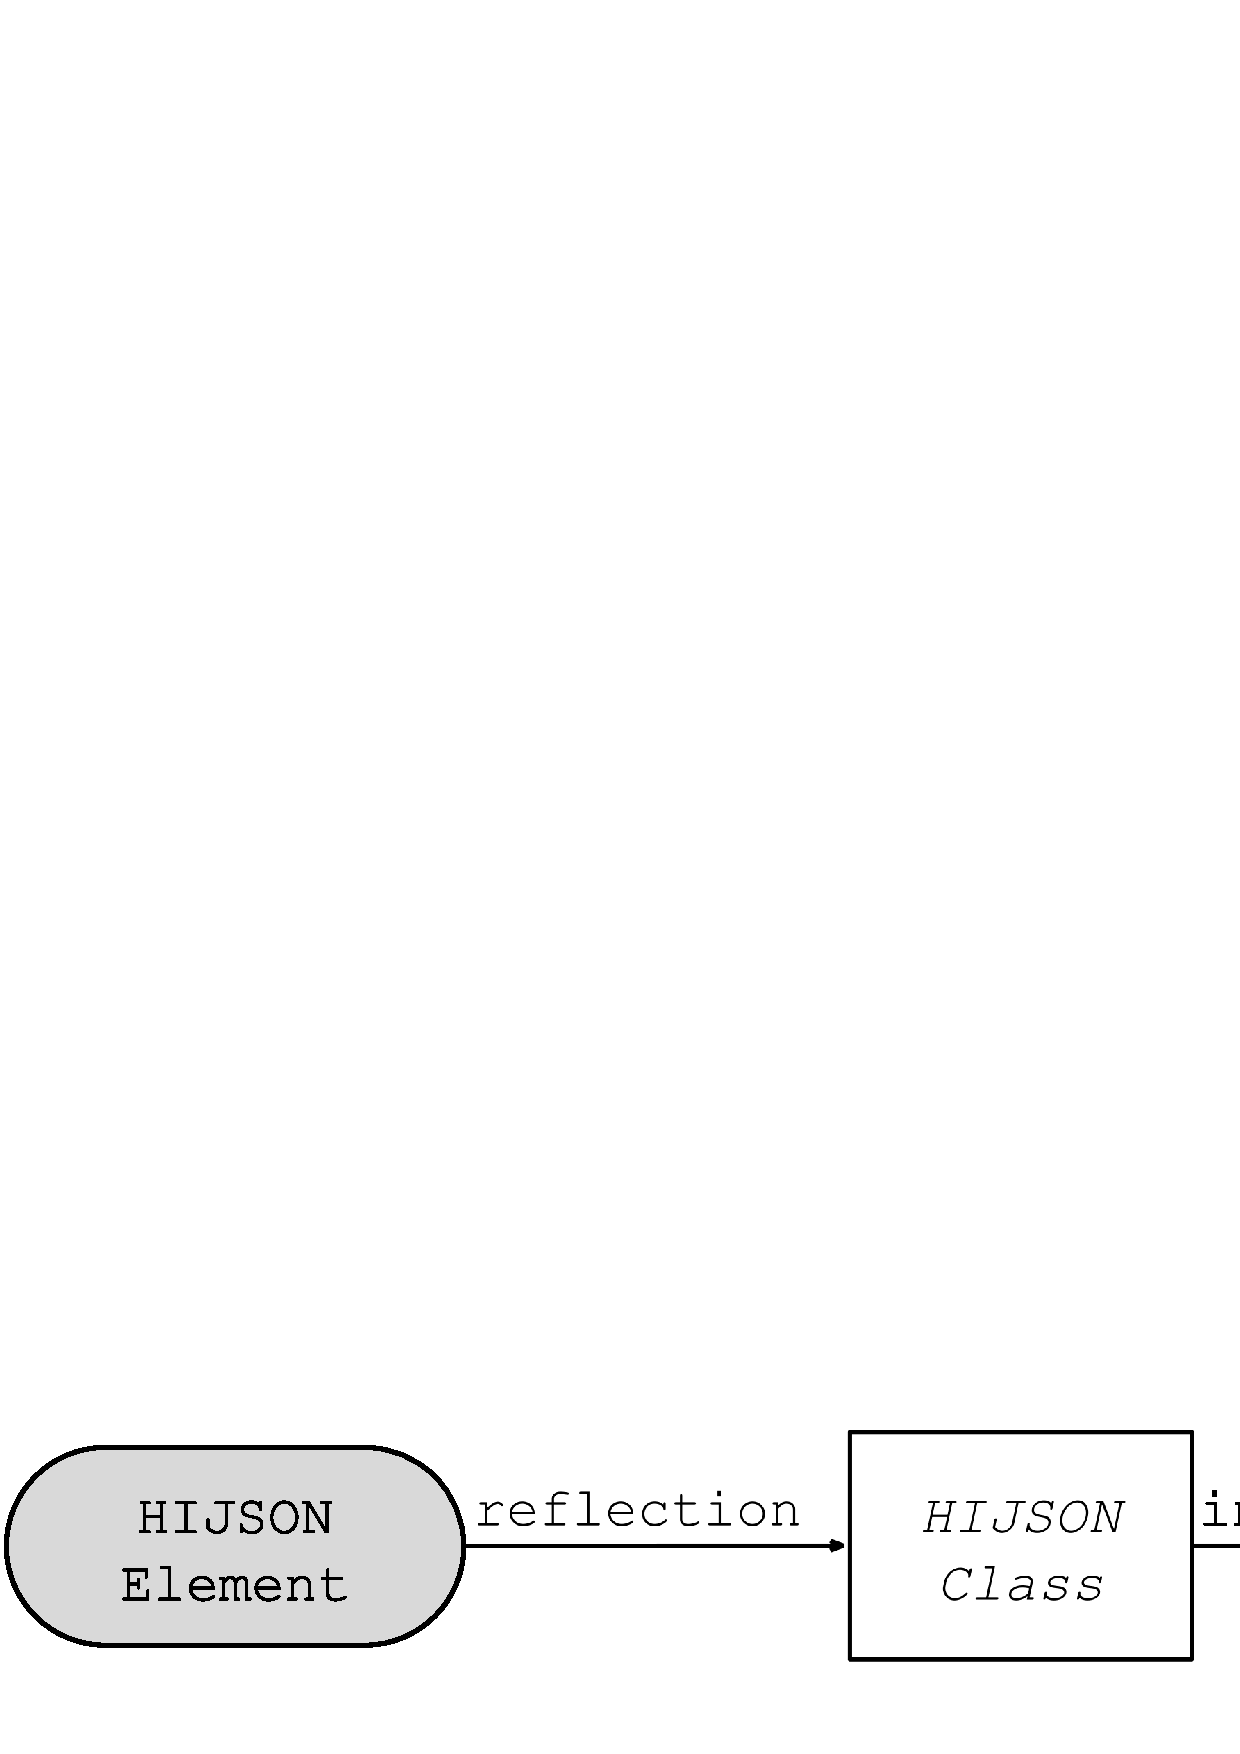
\includegraphics{https://raw.githubusercontent.com/cvdlab/doceng2015/master/images/element-class-node.png}
\caption{``Element/class/node relationship''}
\end{figure}

Each HIJSON Element of the input HJSON document has a dynamic
counterpart inside the toolkit called HIJSON Node, instantiated
according to the relative HIJSON Class through relfection methods (see
picture XXXXX).

To specify a new HIJSON Class means to extend the toolkit to deal with a
new class of HIJSON Element.

To extend the toolkit to deal with a new class of HIJSON Element is
required to to specify a new HIJSON Class, defining the following
properties and methods:

\begin{itemize}
\item
  \texttt{in\_graph}: a boolean value to express if the element is an
  approachable point in the graph paths;
\item
  \texttt{in\_2D\_map}: a boolean value to express if the element is
  wanted in the 2D map;
\item
  \texttt{get2DStyle}: a method that returns the 2D map appearence of
  the element, essentially HTML and CSS code;
\item
  \texttt{get3DModel}: a method that returns the 3D model appearence of
  the element, a THREE.js Object;
\item
  \texttt{getWidget}: a method that returns the information widget, a
  React Component;
\item
  \texttt{getProxy}: a method that returns server side proxy which
  encapsulate IoT sensor communication protocol, a Node.js module.
\end{itemize}

User's needs for new indoor elements, different sensor equipment,
alternative representation on 2D or 3D viewport are accepted by the
definition of new HIJSON Classes that allows in this way single point
custom extension of the toolkit capabilities.

\subsection{Architecture}\label{architecture}

Like the vast majority of the web based application, the toolkit exposes
an overall architecture that is inherently \emph{client/server}. In
particular, two different type of possible client are identifiable: the
\emph{Supervisor} client and the \emph{Explorer} client. Both of them
connect to the same server.

The indoor space described by the HIJSON document provided as input is
processed by the server (cfr. PROCESSING PIPELINE). After that any
connecting \emph{Explorer} client, presumably through a mobile device,
will be provided with the information to perform crossfloor navigation
of the building, while reporting user position to the server. The server
will feed any connecting \emph{Supervisor} client with users positions,
along with data from sensor-equipped things present in the environment,
realizing the IoT monitoring and the realtime multi-person tracking.

\begin{figure}[htbp]
\centering
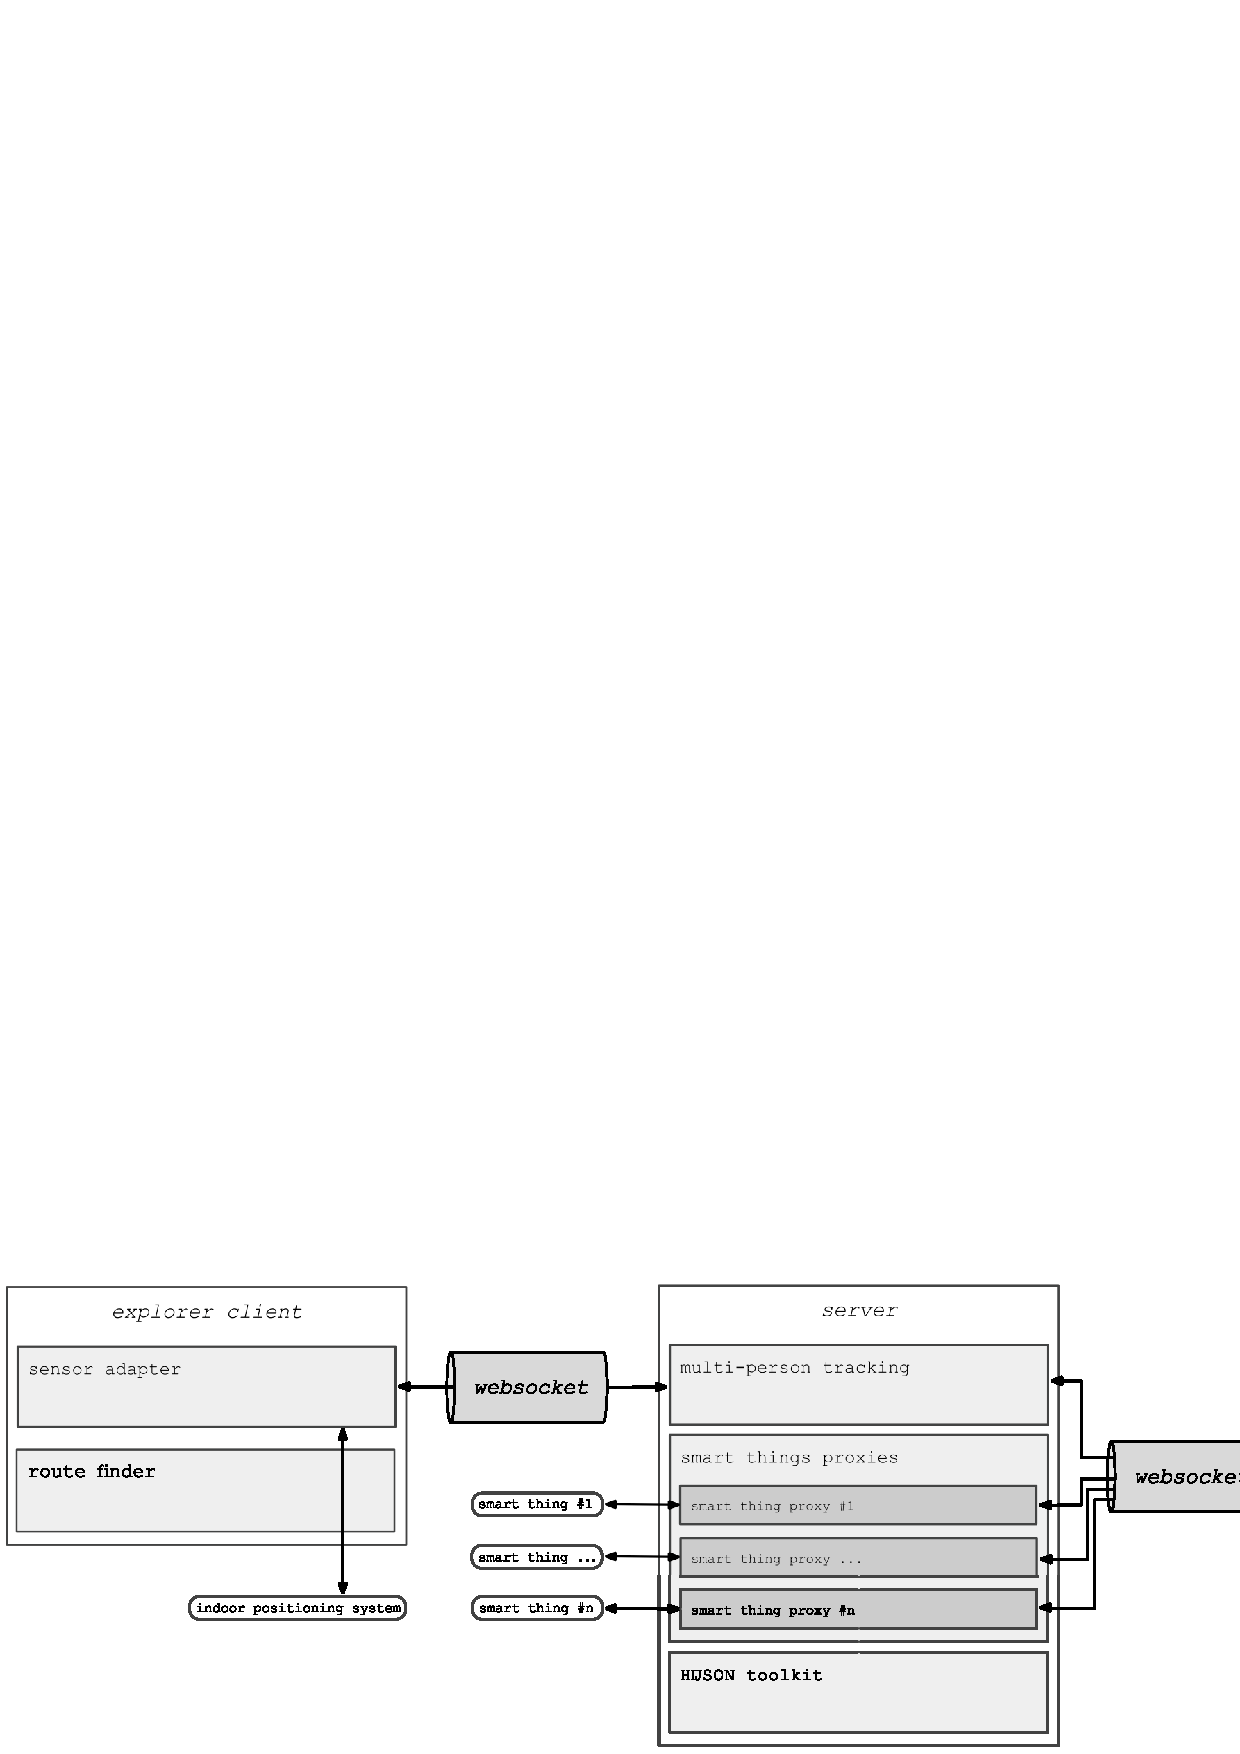
\includegraphics{https://raw.githubusercontent.com/cvdlab/doceng2015/master/images/architecture.png}
\caption{``Architecture''}
\end{figure}

\subsubsection{Server Architecture}\label{server-architecture}

The architecture of the server is depicted in XXXX. A web server module
is responsible for listenning to connecting clients. Each client
connection is handled by the web server module providing all the
required resources and opening one websocket channel, through which will
flow \emph{Explorer} and/or \emph{Supervisor} communication protocol
data. In particular, \texttt{multi-person\ tracking} module receives
position data from \emph{Explorer} clients. It aggregates and sends
these information to connected \emph{Supervisor} clients through the
websocket channel, using a simple but realible protocol later described.
Indipendence from particular IoT sensor equipment communication protocol
is achieved by the \texttt{smart\ things\ proxies} module through the
proxies modules obtained by the HIJSON Class definition
(\texttt{getProxy} method previuosly described).

\subsubsection{\texorpdfstring{Client \emph{Explorer}
architecture}{Client Explorer architecture}}\label{client-explorer-architecture}

The client \emph{Explorer} architecture is generally deployed on a
mobile device, usually supplied to a user who needs to be routed across
the environment described by HIJSON document. The
\texttt{sensor\ adapter} module encapsulates the communication logic
with the indoor positioning system. The presence of this module ensures
indipendece from particularly tecnology allowing client \emph{Explorer}
to rely on different indoor positioning systems: INDICARE ESEMPI SENSATI
E CUTTING EDGE DI POSIZIONAMENTO INDOOR. INTRODURRE IL PROBLEMA DELLA
COMUNICAZIONE A LIVELLO API DEL BROWSER CON SENSORISTICA PER LA
RILEVAZIONE DELLA POSIZIONE.

Every time the \texttt{sensor\ adapter} observe a perceptible
modification in user position sends the new position information to the
server through the single opened websocket, using the a message with the
following syntax:

\begin{verbatim}
currentPosition = {
    coordinates: [x, y],
    levelId: level-ID  
}
\end{verbatim}

Relevant information includes, beside current coordinates, the
indication of the story of the possibly multilevel building the user is
in. The \texttt{smart\ things\ widgets} module being in common with the
client \emph{Supervisor}, has been treated in the next section.

\subsubsection{\texorpdfstring{Client \emph{Supervisor}
architecture}{Client Supervisor architecture}}\label{client-supervisor-architecture}

The Client \emph{Supervisor} architecture shows two modules. The first
one, the \texttt{multi-person\ tracking} module, is responsible to
receive through the websocket, from the server information about
explorers of the environment, showing them in the user interface. The
second module, the \texttt{smart\ things\ widget} communicates with the
server to propose to the user realtime information about sensor-equipped
objects in the environment. Data passes through the single websocket
opened between the server and every \emph{Supervisor} Client. Rely on a
naive but effective communication protocol, each smart thing widget
exchaange data only with respective smart thing proxy on the server. To
ensure the the data is sent only when the user requires the information
relative to a specific smart thing, a widget lifecycle protocol is
implemented: it is based on the 4 events \texttt{on\_before\_show},
\texttt{on\_show}, \texttt{on\_before\_hide}, \texttt{on\_hide}
triggered, as suggested by their names when a widget is shown or hidden.
When the user requires information about a smart thing, its widget has
to be rendered, but \texttt{on\_before\_show} the server is notified to
connect via relative proxy to the sensor. Once connected, the server
begin to send data via webscocket. Received data is shown through the
wodget to the user. When done, or \texttt{on\_before\_hide} event of the
widget, a notification is sent to the server announcing to stop sending
data and the proxy close the connection to the sensor. Widget lifecycle
protocol ensures that only requiring data is sent from th eserver to the
client.

\subsection{HIJSON processing
pipeline}\label{hijson-processing-pipeline}

Each time a new HIJSON document is submitted to the server, it is passed
through the \textbf{HIJSON processing pipeline}, where it is subjected
to a sequence of preliminary transformations.

The application of the transformation pipeline has a double aim. The
first one consists in generating the graph of valid paths between all
the interesting HIJSON elements. The second aim is the generation of one
\emph{GeoJSON} document for each story of the building described by the
HIJSON document. In this way any connected client can be provided with a
bidimensional plant for each level of the building that it can visualize
through any compliant GeoJSON viewer.

HIJSON processing pipeline (as pictured in figure AGGIUNGERE
RIFERIMENTO) is composed by 6 elaboration stages. In the following are
detailed operations excecuted by each stage, which are, in the order:
\emph{validation}, \emph{georeferencing}, \emph{parsing}, \emph{graph
paths generation}, \emph{2D layers generation}, \emph{marshalling}.

\begin{figure}[htbp]
\centering
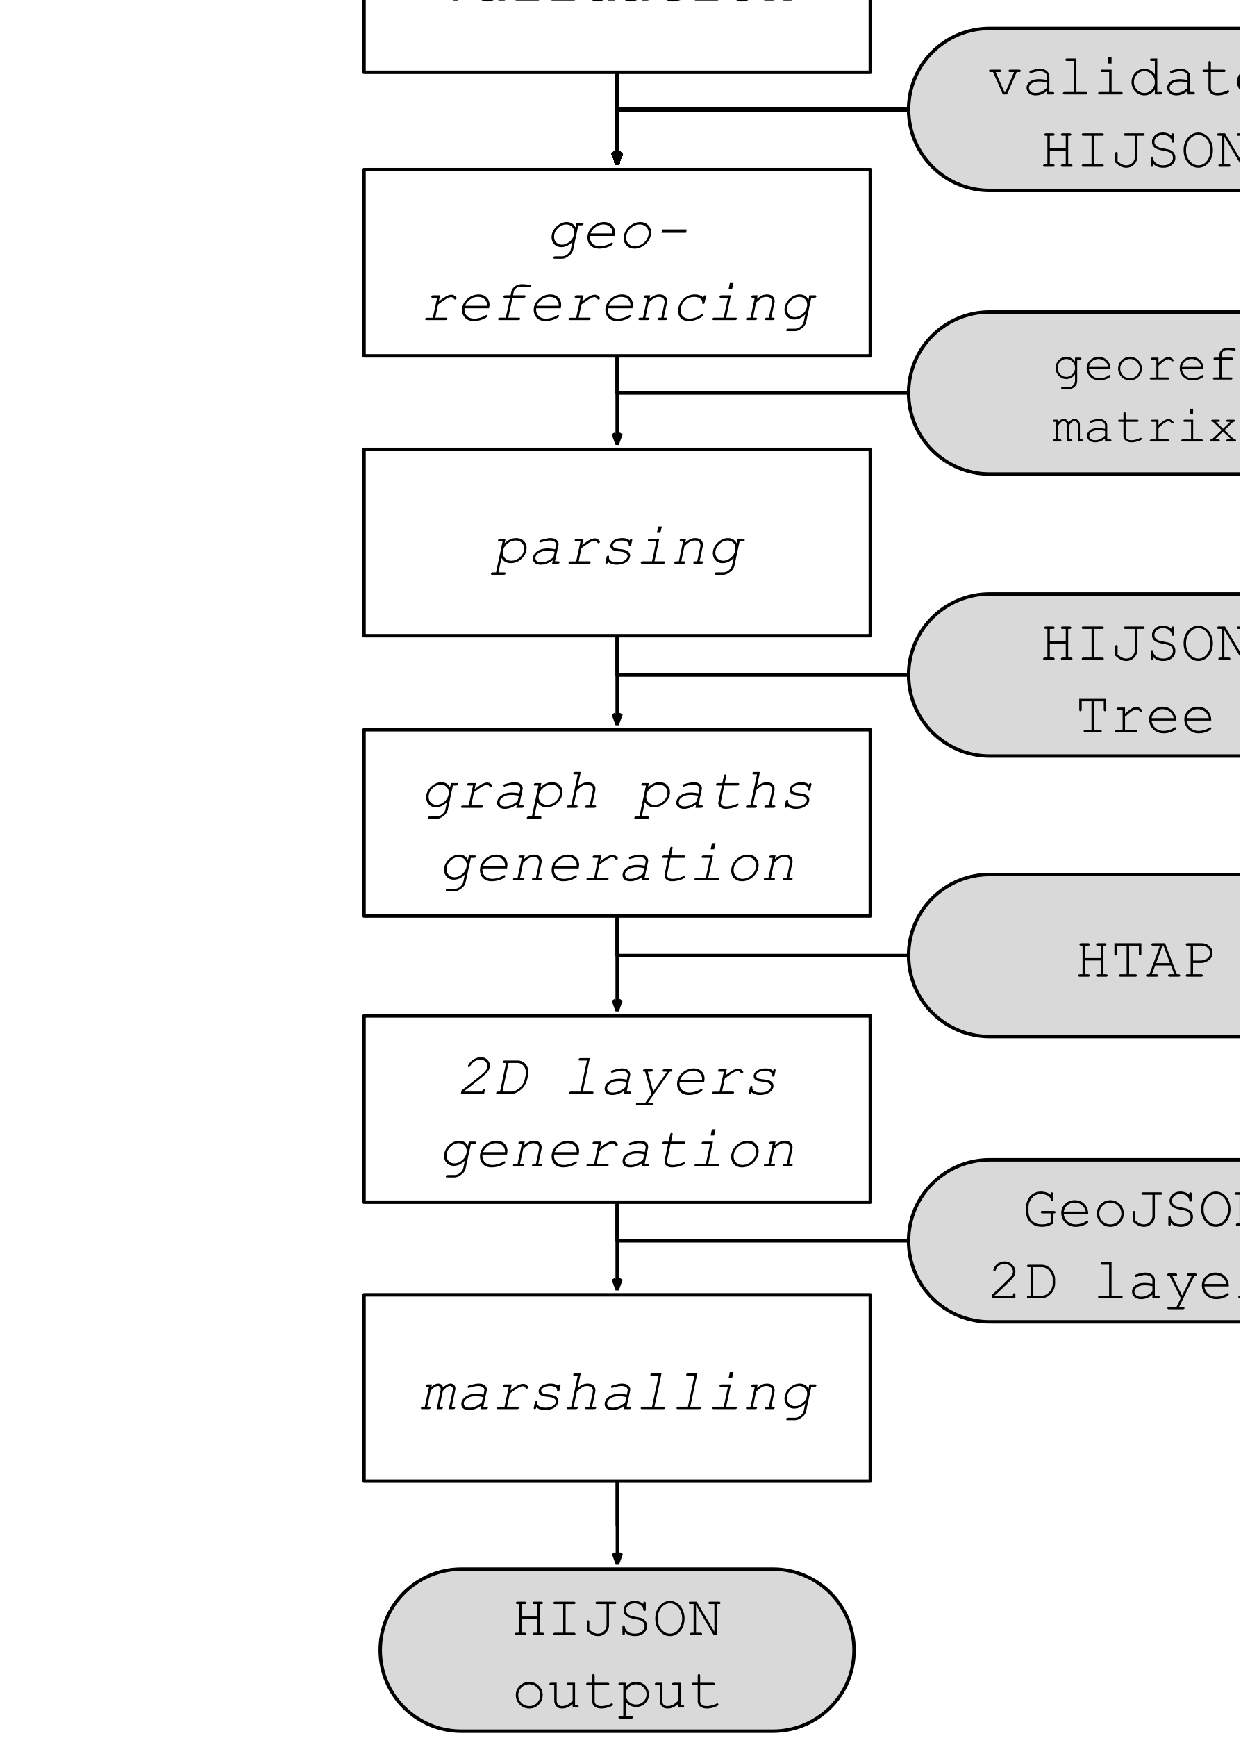
\includegraphics{https://raw.githubusercontent.com/cvdlab/doceng2015/master/images/pipeline.png}
\caption{``HIJSON processing pipeline''}
\end{figure}

\begin{enumerate}
\def\labelenumi{\arabic{enumi}.}
\itemsep1pt\parskip0pt\parsep0pt
\item
  {[}\textbf{validation}{]} - The first one is the validation stage. In
  order to begin with the effective transformations the input HIJSON
  document must be compliant with the rules defined in (AGGIUNGERE REF
  TO PARAGRAFO REGOLE DI VALIDITA'). In the case the validation stage
  fails, processing aborts and do not continue to following stages. If
  the stage success, the output for the next stage is a validated
  HIJSON.
\item
  {[}\textbf{georeferencing}{]} - In the second stage, in order to allow
  for continuous outdoor/indoor navigation, the system needs to compute
  the georeferencing matrix, a linear operator able to transform local
  coordinates into global coordinates (referred to world coordinate
  system as latitude and longitude misures) and viceversa. This task is
  accomplished by solving a linear system obtained from information
  contained in HIJSON configuration part and precisely from the
  correnspondance of three real word points to three points included
  into the HIJSON document.
\item
  {[}\textbf{parsing}{]} - The parsing stage, takes the validated and
  georeferenced HIJSON as its input, that as illustrated before can be
  thought of as a list of HIJSON Elments, parses them and produce an
  istance of HIJSON Tree. The HIJSON Tree is an object in memory
  representing the tree hierarchical structure of the building described
  by the HIJSON document.
\item
  {[}\textbf{graph paths generation}{]} - The fourth stage is in charge
  of the generation of the graph paths. This aim is accomplished
  according to the algorithm described in (AGGIUNGERE RIFERIMENTO A
  \#\#\#\# Automatic generation of valid paths). The graph paths will be
  useful afterwards to coumpute valid paths from couple of point of
  interest on the graph. Once the graph paths has been computed, the
  input HIJSON Tree is augmented with paths information, becoming what
  has been called an HTAP (HIJSON Tree Augmented with Paths).
  Augmentation always takes place as leaf nodes added as children of a
  specific (e.g. ``room'') level.
\item
  {[}\textbf{2D layers generation}{]} - The fifth stage is the
  generation of GeoJSON layer. For each level, the system generates one
  geoJSON layer that will be use for the creation of 2D map. Each layer
  contains the children of `level' node in the HIJSON Tree. Every class
  contains a boolean value that is used to choose which class will be a
  part of geoJSON layer. Every element has a geographical coordinates
  calculated by the transformation matrix with regard to the local
  coordinates of the HIJSON element.
\item
  {[}\textbf{marshalling}{]} - The last stage is responsible of execute
  a serialization of the the transformed data. Tasks like breaking
  dependency-loops and stringification are performed, and the output is
  stored ready to be served to any requiring client.
\end{enumerate}

\subsubsection{Algorithmics: automatic generation of valid
paths}\label{algorithmics-automatic-generation-of-valid-paths}

(IN QUESTA SEZIONE SI POSSONO AGGIUNGERE EVENTUALI APPROFONDIMENTI DI
ALTRI STADI DELLA PIPELINE)

The fourth stage of the processing pipeline is responsible for the
generation of a graph of valid paths through the entire model
represented by the intput HIJSON document. The graph generated according
to the algorithm described in the following, although not optimal,
ensures a complete coverage of the surface while limiting the numebr of
generated nodes. Resulting graph is weigthed on the edges with nodes
distances and each node represents alternatively:

\begin{enumerate}
\def\labelenumi{\alph{enumi}.}
\itemsep1pt\parskip0pt\parsep0pt
\item
  standard path node, i.e.~a junction node or possibly an endpoint of a
  path;
\item
  connection node, used as subproblem composing element in the divide et
  impera approch adopted (as described below).
\item
  element nodes ie. HIJSON Element (whose HIJSON Class explicitly grants
  his presence in the graph), typically an endpoint of a path;
\end{enumerate}

Such a graph allows for directions calculations between any two given
nodes. Directions are actually computed clientside applying the
Dijkstra's shortes route algorithm on the graph.

Taking advantage of the hierarchical structure of the HIJSON document,
and according to the divide et impera approach, the problem of the graph
paths generation is splitted in several sub-problems which consist in
the computation of the sub-graphs relative to each room, or more
generally ambience. The sub-graphs are then linked together through the
connection nodes (which in most cases represents doors). The resolution
of each sub-problem (as depicted in figure METTERE RIFERIMENTO ALLA
FIGURA), is composed by 4 phases:

\begin{enumerate}
\def\labelenumi{\arabic{enumi}.}
\itemsep1pt\parskip0pt\parsep0pt
\item
  Computation of the walkable area of the ambience: this task is
  accomplished subtracting area of the possibly encumbrances to the area
  of the ambience; the result is tipically a surface with holes;
\item
  Triangulation of the walkable area: the computed surface is
  triangulated taking into account the presence of holes;
\item
  Identification of graph nodes: for each triangle side completely
  internal to the area, its midpoint is selected as standard path node;
\item
  Junction of nodes: nodes relative to the same triangle are then linked
  together; both element nodes and connection nodes (i.e.~doors) are
  linked to the nearest node in the ambience (i.e.~room).
\end{enumerate}

\begin{figure}[htbp]
\centering
\includegraphics{https://raw.githubusercontent.com/cvdlab/doceng2015/master/images/graph-generation/single/graph-generation-1.png}
\caption{``Graph generation: 1. computation of the walkable area''}
\end{figure}

\begin{figure}[htbp]
\centering
\includegraphics{https://raw.githubusercontent.com/cvdlab/doceng2015/master/images/graph-generation/single/graph-generation-2.png}
\caption{``Graph generation: 2. triangulation of walkable area''}
\end{figure}

\begin{figure}[htbp]
\centering
\includegraphics{https://raw.githubusercontent.com/cvdlab/doceng2015/master/images/graph-generation/single/graph-generation-3.png}
\caption{``Graph generation: 3. identification of graph nodes area''}
\end{figure}

\begin{figure}[htbp]
\centering
\includegraphics{https://raw.githubusercontent.com/cvdlab/doceng2015/master/images/graph-generation/single/graph-generation-4.png}
\caption{``Graph generation: 4. junction of nodes''}
\end{figure}

\section{Conclusions}\label{conclusions}

We presented HIJSON a GeoJSON extension for indoor mapping TRA GLI
SVILUPPI FUTURI: - GENERAZIONE GRAFICA IN AMBIENTE CAD DEL DOCUMENTO
HIJSON

\section{Bibliography}\label{bibliography}

\end{document}
